\newcommand{\labname}{Lab 3}
\documentclass[11pt]{article}
\usepackage[left=1in, right=1in, top=1in, bottom=1in]{geometry}
\usepackage{amsmath,amsfonts,amssymb}
\usepackage{graphicx}
\usepackage{fancyhdr}

% TODO: CHANGE THESE
\newcommand{\myname}{Alex Miller} % Full Name
\newcommand{\mycnetid}{amiller68} % CNetID

% header
\pagestyle{fancy}
\fancyhf{}
\lhead{CS 162 \labname}
\chead{\myname{} (\mycnetid)}
\rhead{Page \thepage{} of \pageref{mylastpagelabel}}

% document starts
\begin{document}

\paragraph{Task 5.1} Message      	 : NSA IS  CIA IS  IRA
\newline Key   			 : LA  CHI CIA
\newline Encrypted Message: LA  PW  IRA CIA WIFI

\paragraph{Task 5.2} 
Find the value of i \% $\ell$, call it keyIndex.
\newline ${w_c}_i$ = ${w_m}_(i+keyIndex)\%$\ell$$

\paragraph{Task 5.3}
\newline ${w_m}_i$ = ${w_c}_($\ell$+(i-keyIndex))\%$\ell$$

\paragraph{Task 7.1}
\begin{figure}[htbp]
 \begin{center}
  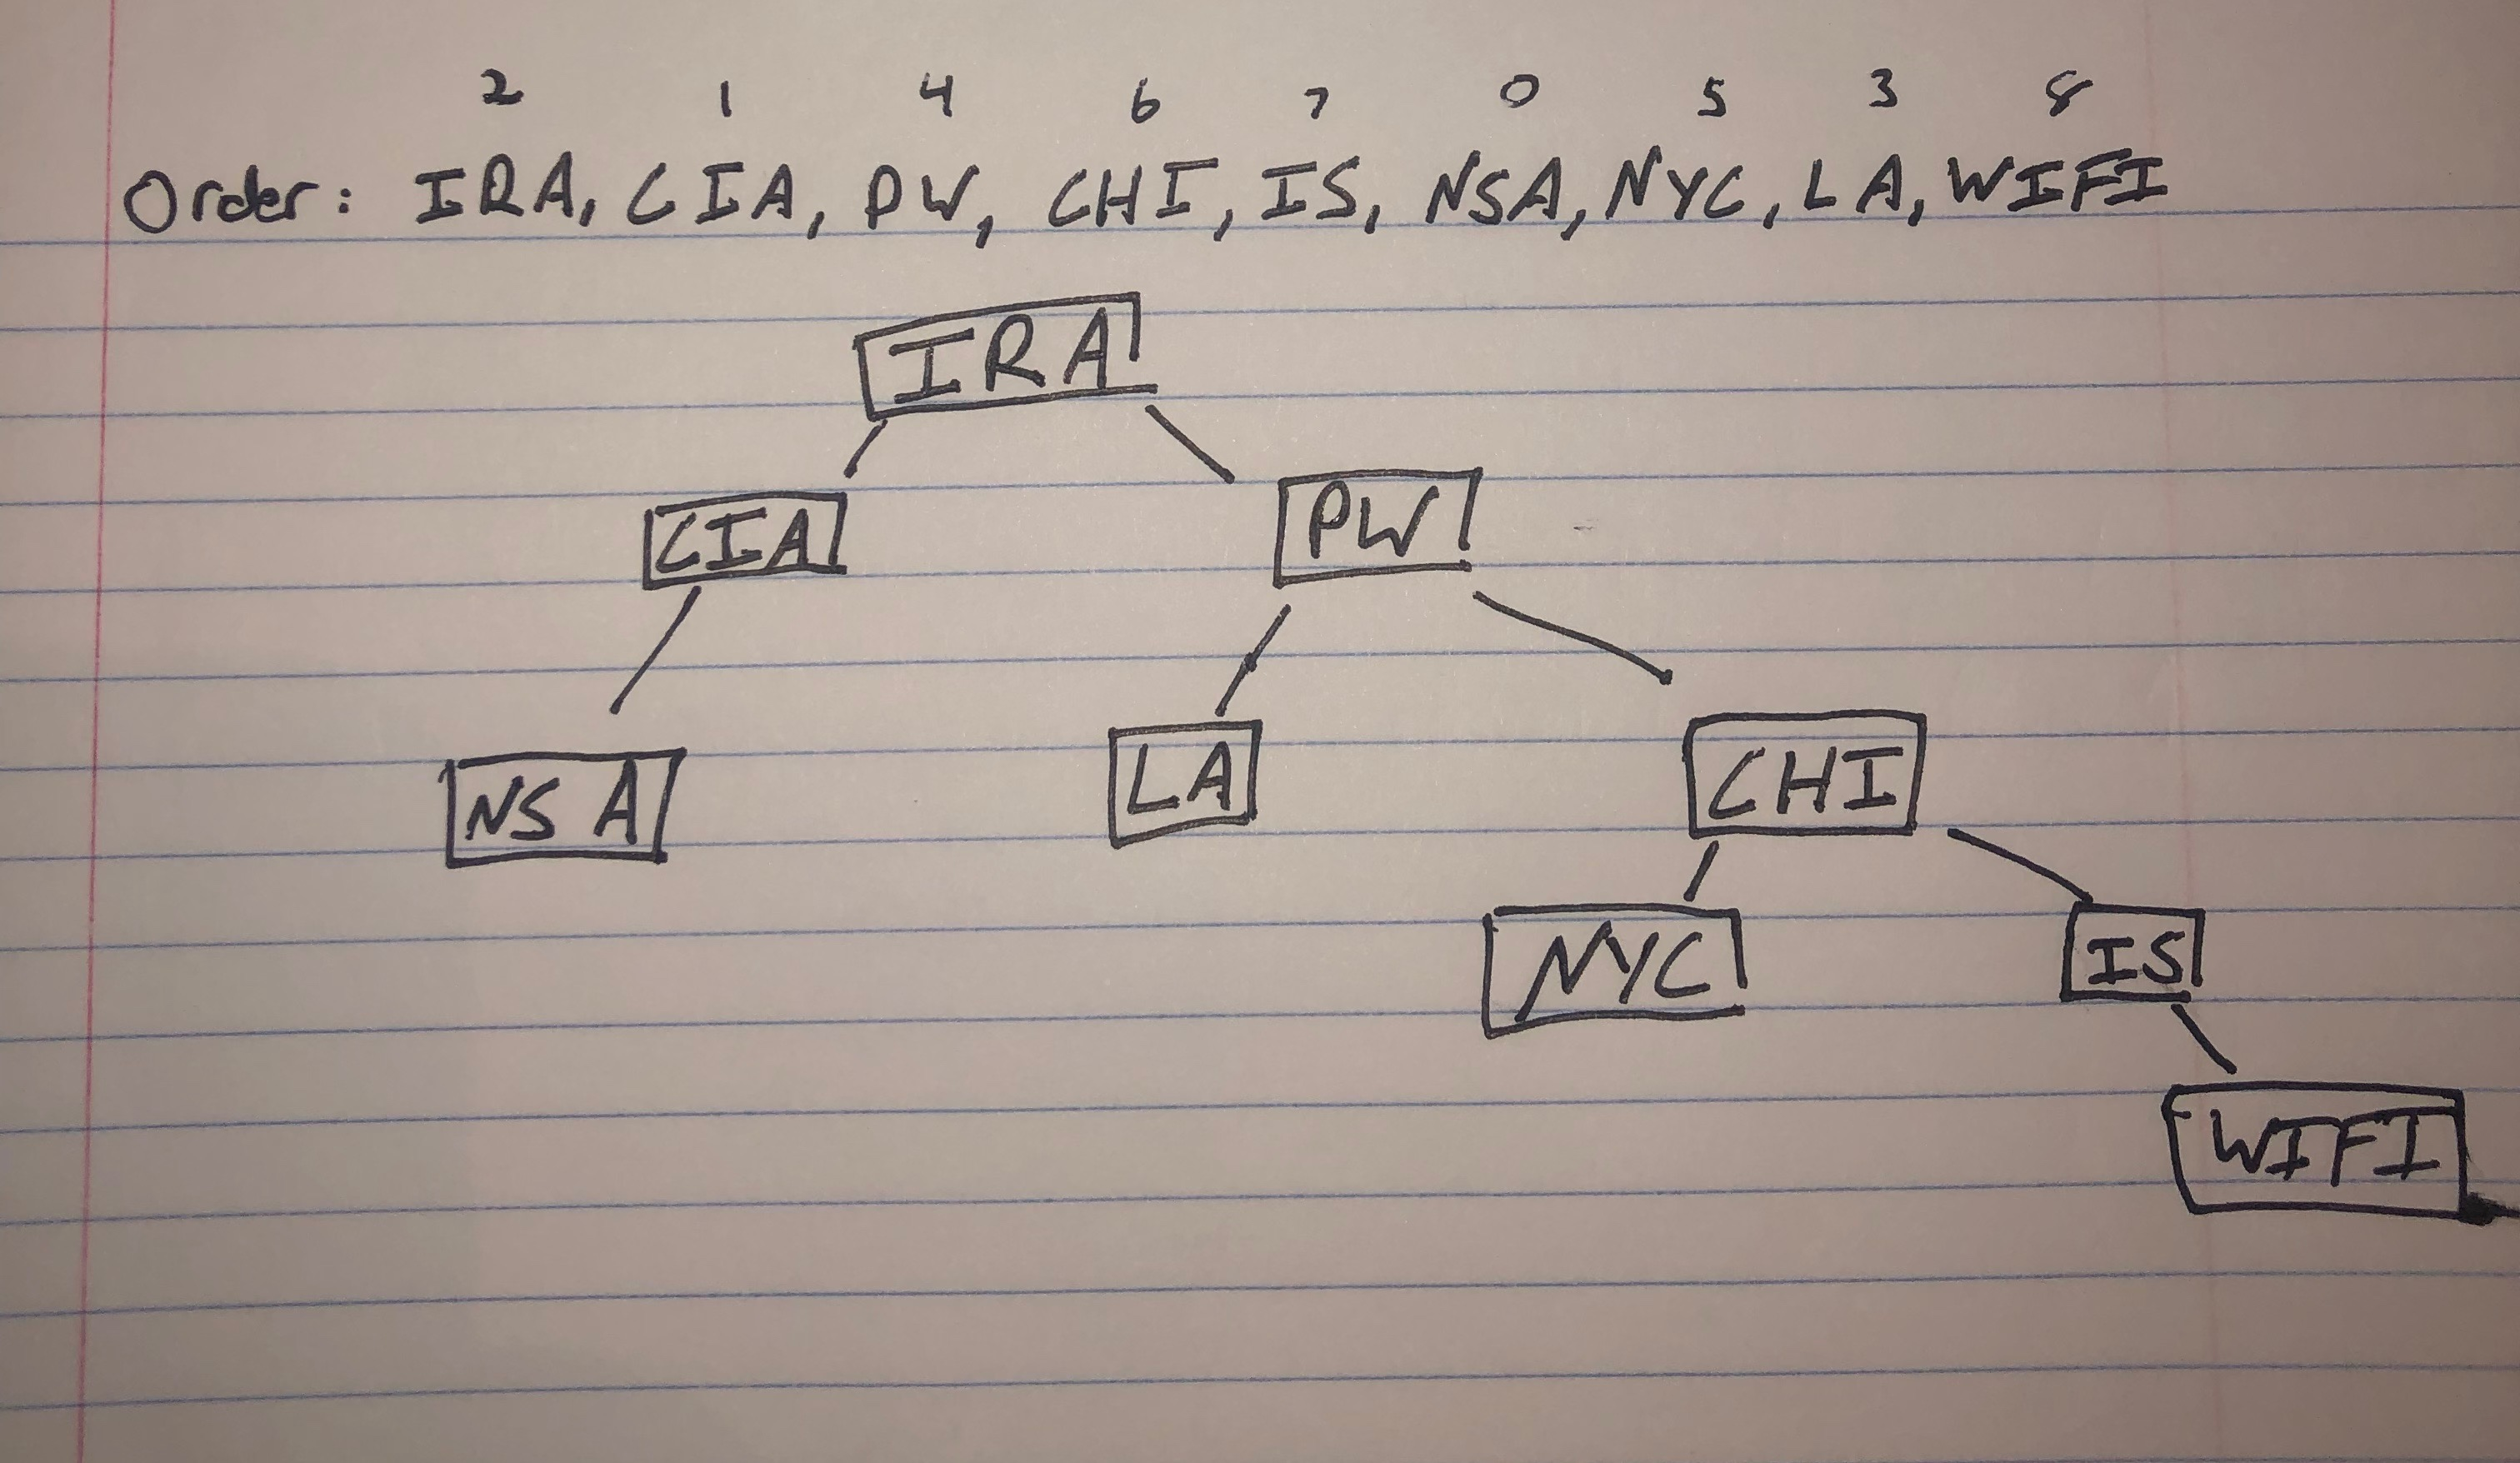
\includegraphics[width=0.5\textwidth]{7_1.JPG}
  \caption{Task 7.1}
 \end{center}
\end{figure}


\paragraph{Task 7.2} \newline

\newline First Blank : 0
\newline Second Blank: num\_trees(i) * num\_trees(n-i-1) 

\paragraph{Task 7.3}
Field to be added: i`nt size;
\newline The field represents the size of the tree rooted to a given node. Every time a new node is inserted into a tree the size of that tree is incremented

\paragraph{Task 7.4}
The Solution has a runtime that is proportional to Log N (where N is the number of Nodes in the tree) because (in the average case) that is the number of steps it takes to reach a leaf of the tree from the root of the tree. 
\newline First Blank 
\newline		 	   T \rightarrow adress = addr; 
\newline 			   T \rightarrow distance = dist;
\newline			   T \rightarrow price = price;
\newline 			   T \rightarrow left = NULL;
\newline			   T \rightarrow right = NULL;
\newline 			   T \rightarrow size = 1;
\newline
\newline Second Blank 
\newline		   	   T \rightarrow left = insert(T \rightarrow left, addr, dist, price);
\newline			   T \rightarrow size ++;
\newline
\newline Third Blank  
\newline		       T \rightarrow right = insert(T \rightarrow right, addr, dist, price);
\newline			   T \rightarrow size ++;

\paragraph{Task 7.5}
Search Protocol of range(T, d1, d2);
\newline If T == NULL, return 0. Otherwise Proceed to step 0
\newline Step 0:
\newline Look at the distance stored in the tree. If is greater than d2, run the search protocol on the left subtree (return range(T \rightarrow left), d1, d2)). If it is less than d1, run the search protocol on the right tree (return range(T \rightarrow right, d1, d2)). If it is greater than or equal to d1 and less than or equal to d2 proceed to step 1.
\newline Step 1
\newline Store the size of the tree in a value called size%_total and proceed to step 1a.
\newline Step 1a
\newline Continue moving down the left edge of the tree until you encounter a node that is less than d1. Subtract the size field of this node form size%_{total}. 
Go to the left child of the tree. If it's distance is equal to d1, subtract the size of its left child from size%_exp{total} and go to step 2. If it greater than d1 repeat step 1a. If it is less than d1 proceed to step 1b.
\newline Step 1b
\newline Subtract the size of this subtree from size%_exp{total}. Go down the right child of the tree, call this tree right. add the value of range(right, d1, d2) to the value of size_total. Proceed to step 2a.

\newline Look for the first value that 
\newline Search the tree for the first value less than the lower end of the range
\newline The reason this runs in Log(N) time is because it only makes two paths down the tree, which each take log


\paragraph{Task 8.1}
\begin{figure}[htbp]
 \begin{center}
  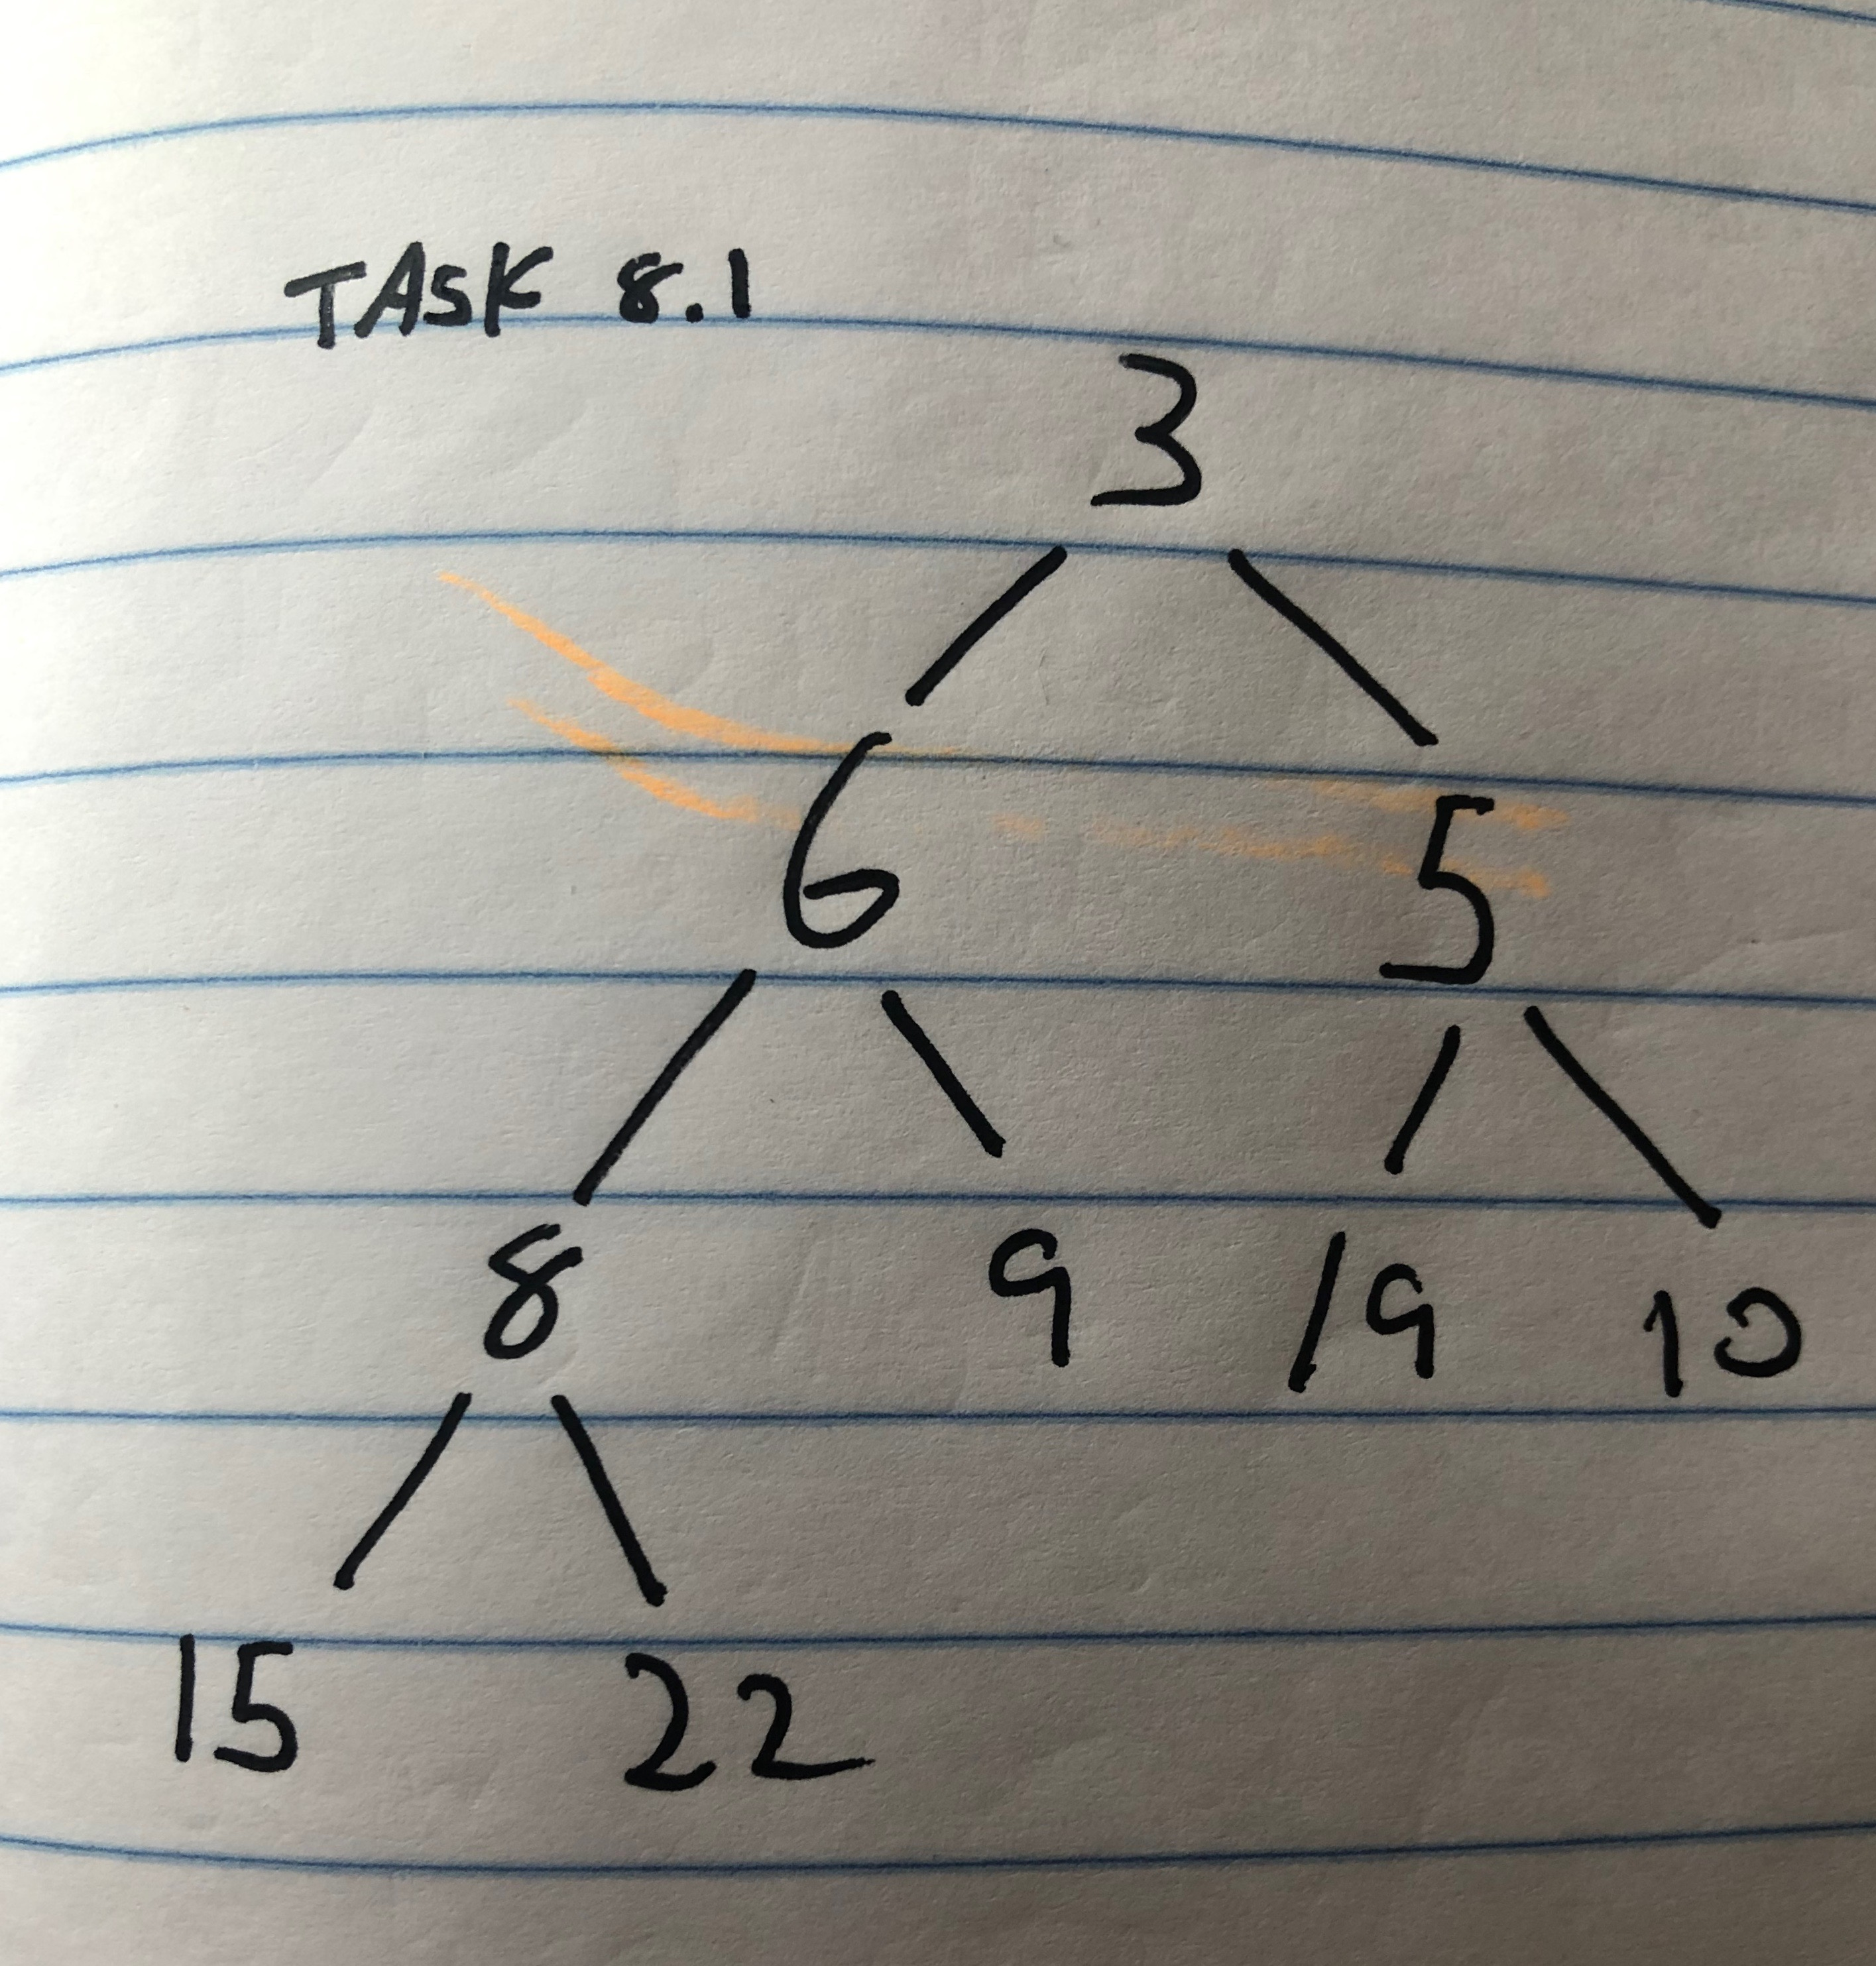
\includegraphics[width=0.5\textwidth]{8_1.JPG}
  \caption{Task 7.1}
 \end{center}
\end{figure}


\paragraph{Task 8.2}
\begin{figure}[htbp]
 \begin{center}
  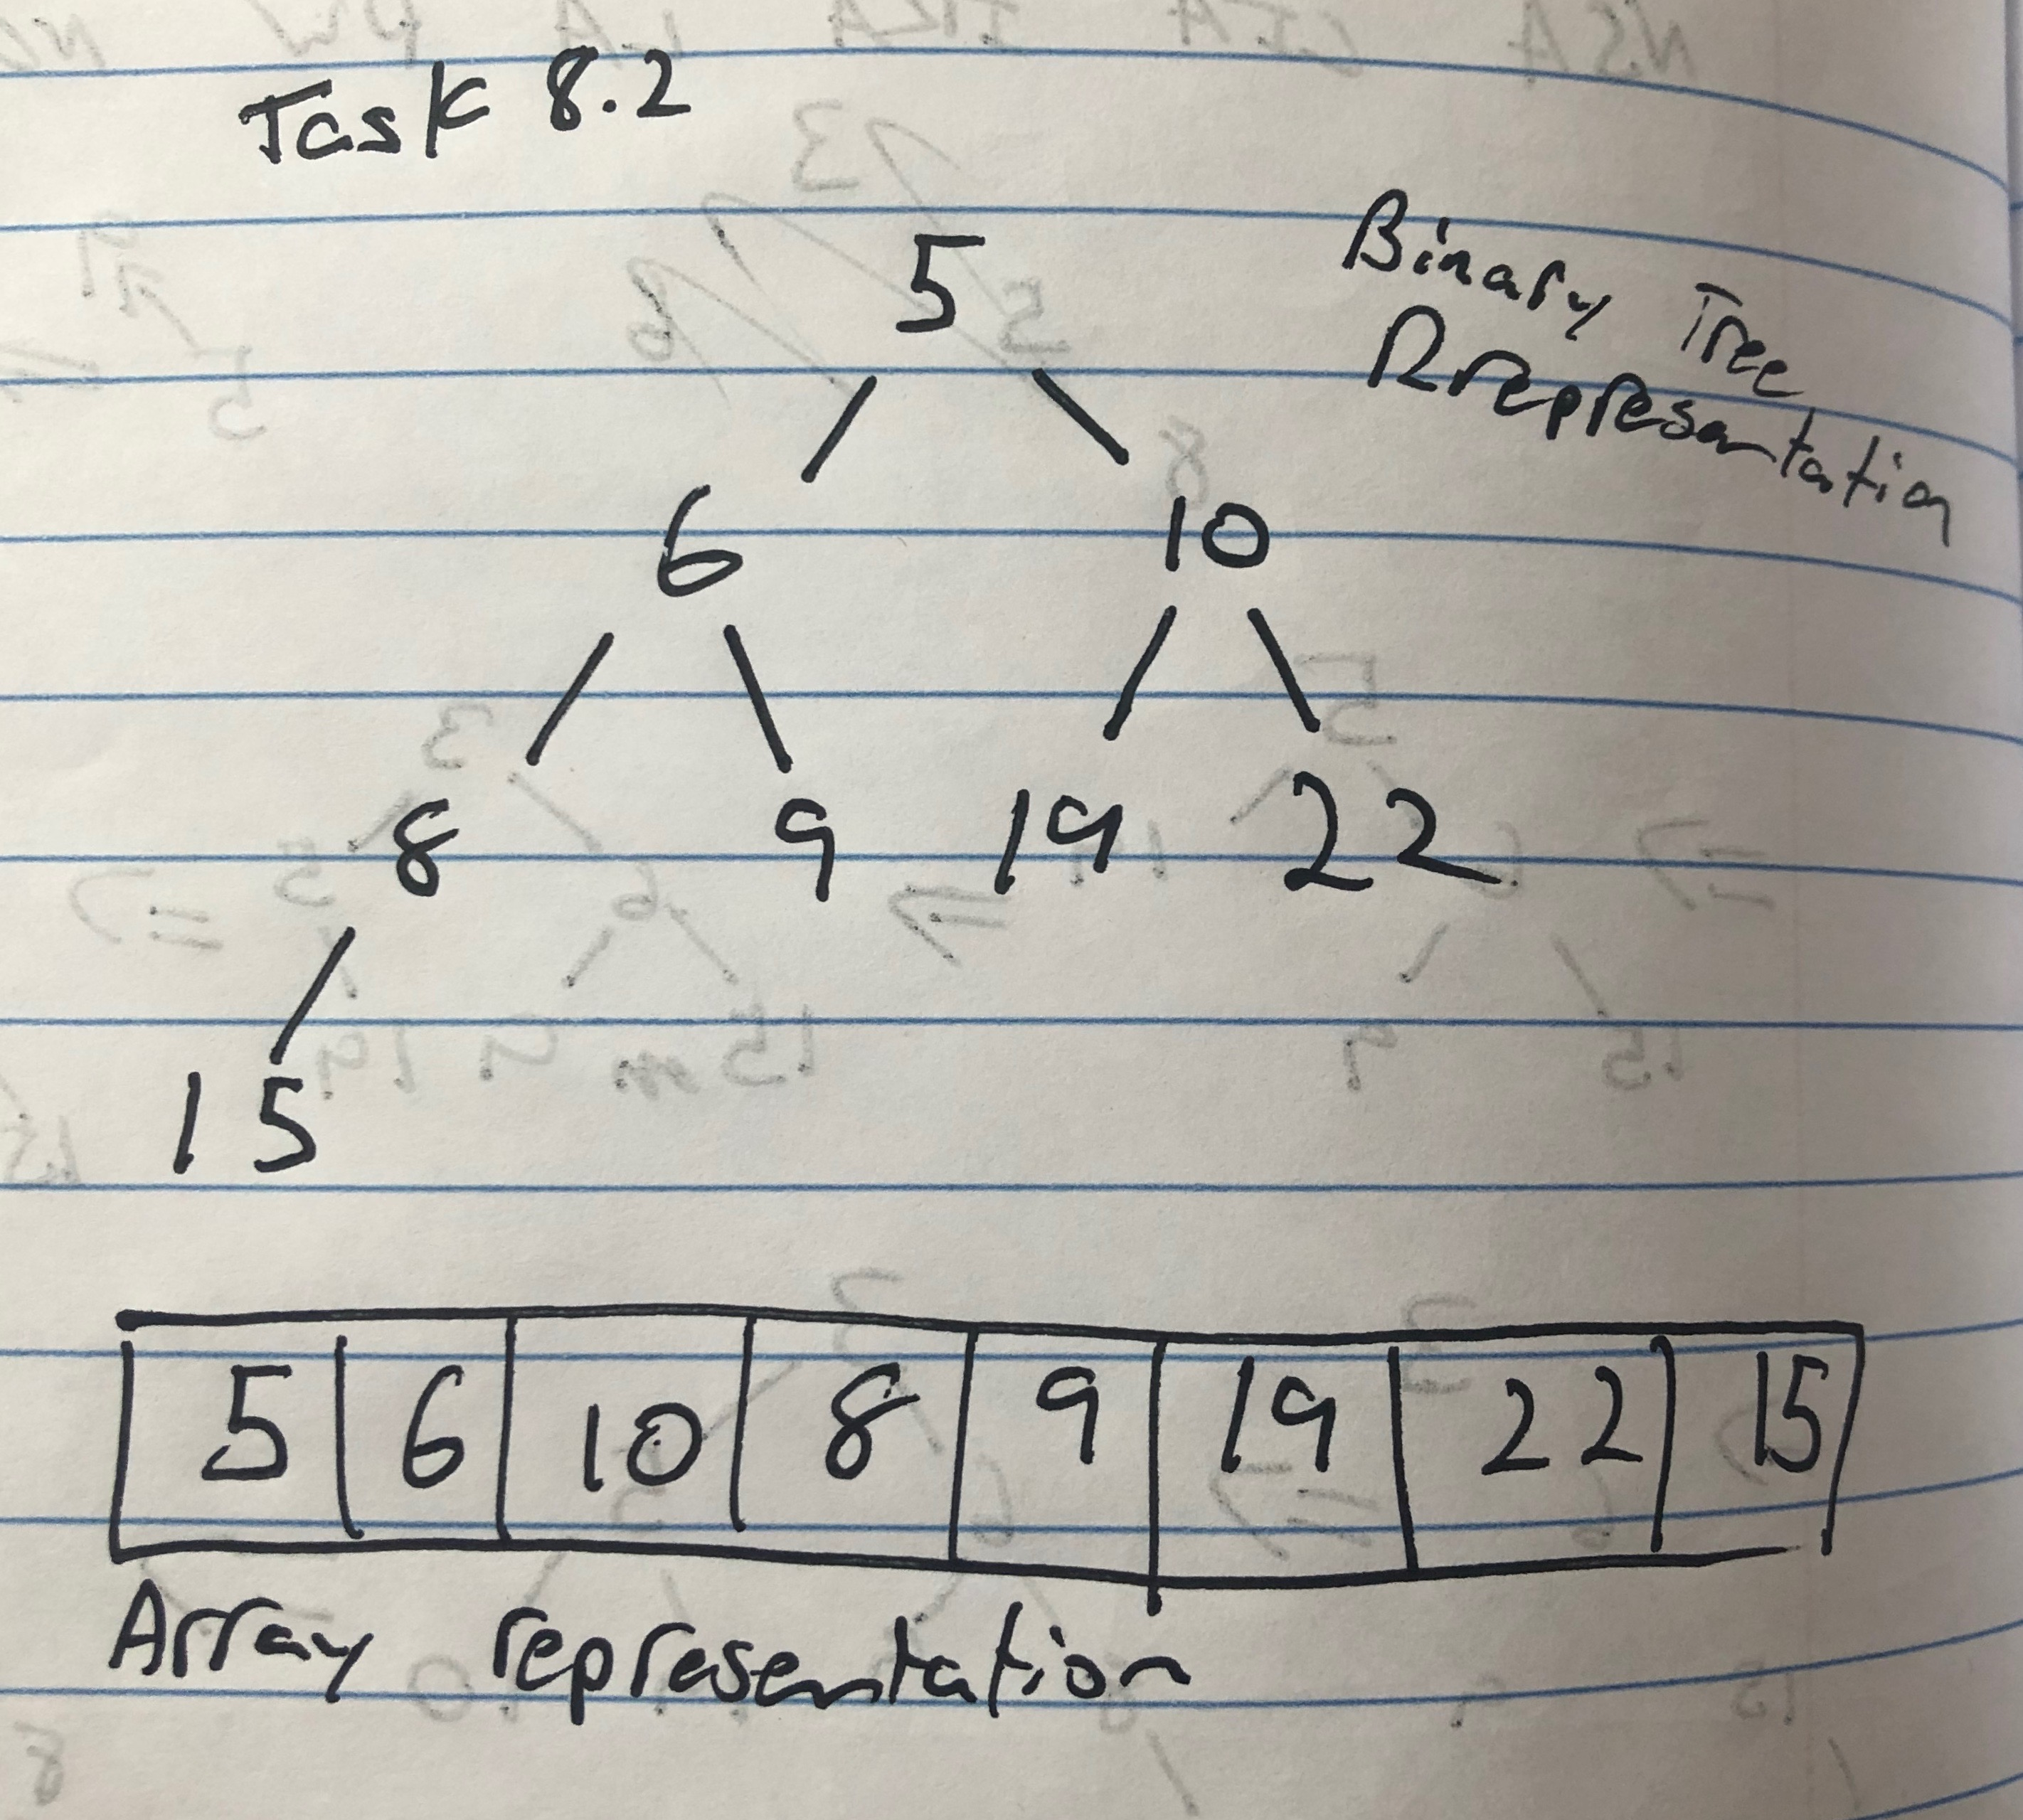
\includegraphics[width=0.5\textwidth]{8_2.JPG}
  \caption{Task 7.1}
 \end{center}
\end{figure}

\paragraph{Task 8.3}
\begin{figure}[htbp]
 \begin{center}
  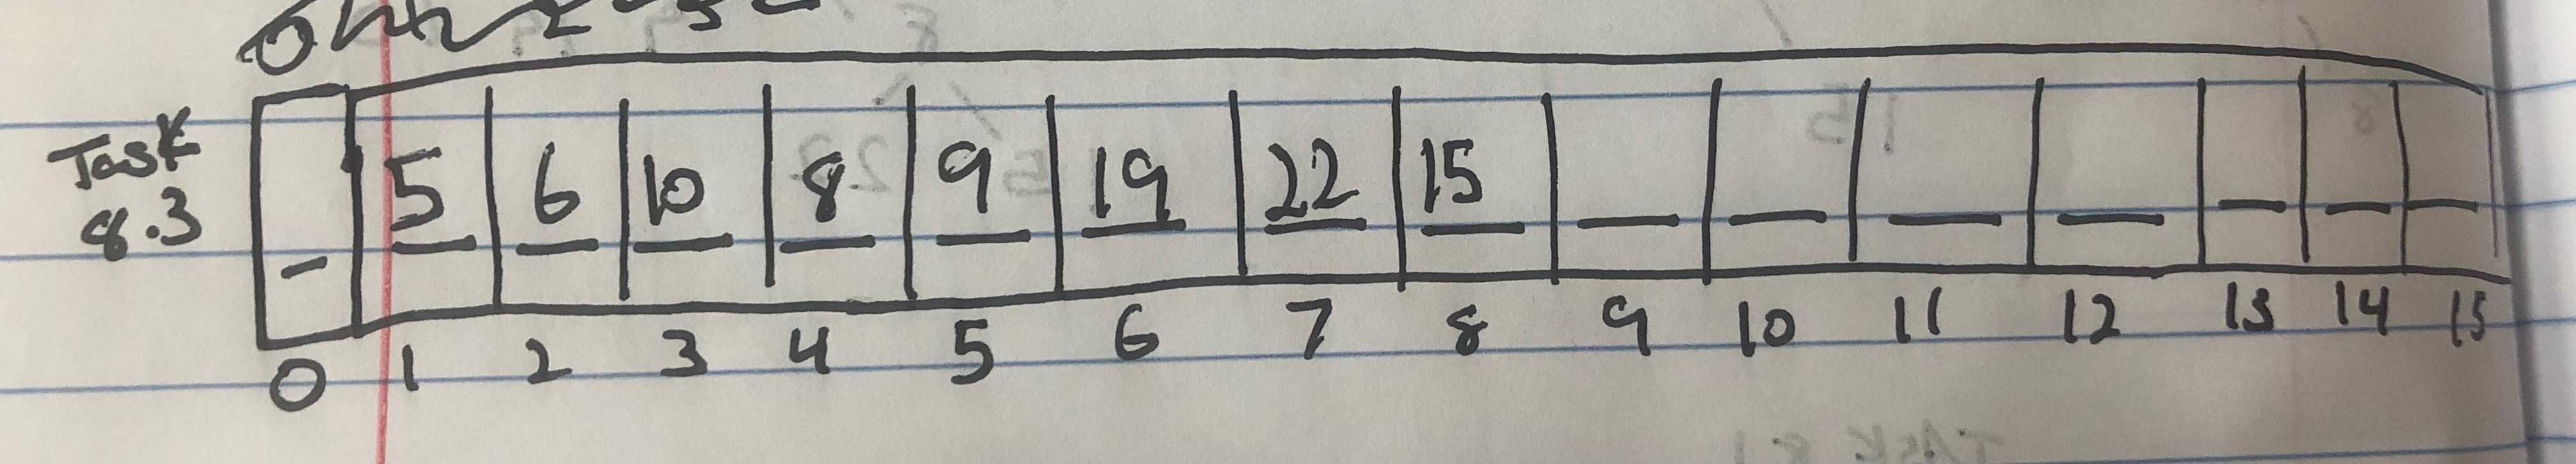
\includegraphics[width=0.5\textwidth]{8_3.JPG}
  \caption{Task 7.1}
 \end{center}
\end{figure}

\paragraph{Task 8.4}
\newline First Blank : p \textless \left( H \rightarrow priorities \right) \lbrack idx \rbrack || idx \textgreater size
\newline
\newline Second Blank: p == (H \rightarrow priorites) \lbrack idx \rbrack
\newline 
\newline Third Blank : 
\newline
\newline Foruth Blank: return (heap%_search(H, p, 2*idx) || heap_search ( H, p, 2*idx+1 )
\newline

\paragraph{Task 8.5}
\newline The data structure has three fields. The first one is a median value. The last two are two heaps, a min heap and a max heap. Every element in the min heap is greater than or equal to the median. Every element in the max heap is less than the median.
\newline Track the size of both heaps.
\newline Finding the median involves the follwing steps:
\newline Get the value of the median field stored the the structure. This has O(1) time because it is just looking up a value at a known location.
\newline Deleting the median involves the following steps:
\newline If the sizes of the two heaps are equal, make the median field equal the min value of the min heap. Delete the min value of the min heap. If the size of the min heap is greater than the size of the max heap, make the median field equal the min value of the min heap. Delete the min value of the min heap. If the size of the max heap is greater than the size of the min heap, make the median field equal the max value of the max heap. Delete the max value of the min heap. Delete only takes O(Log N) time because it only involves deleting root value from heaps, which has O ((Log N)/2) complexity.





\label{mylastpagelabel}

\end{document}
